\documentclass{BHCexam}	
\newcommand{\xl}[2]{\vv{#1}\bm\cdot\vv{#2}}
\newcommand{\zj}[1]{\vspace{-1em}\begin{center}\begin{tikzpicture}#1\end{tikzpicture}\end{center}}
\begin{document}
\begin{questions}

\qs 已知平面上三点$ A,~B,~C $满足$ \abs{\vv{AB}}=6,~\abs{\vv{AC}}=8,~\abs{\vv{BC}}=10,~ $则$ \vv{AB}\bm{\cdot}\vv{BC}+\vv{BC}\bm{\cdot}\vv{CA}+\vv{CA}\bm{\cdot}\vv{AB}= $\xx
\onech{$ 48$}{$ -48$}{$ 100$}{$ -100$}
\qs 在三角形$\triangle ABC$中,点$ D $满足$ \vv{AD}=2\vv{AB}-\vv{AC} $,则\xx
\twoch{点$ D $不在直线$ BC $上}{点$ D $在$ BC $的延长线上}{点$ D $在线段$ BC $上}{点$ D $在$ CB $的延长线上}
\qs 
如图,在等腰梯形$ ABCD $中,$ AB=8,~BC=4,~CD=4,~ $点$ P $在线段$ AD $上运动,则$\left|\vv{PA}+\vv{PB}\right| $的取值范围是\xx
\onech{$ \left[6,4+4\sqrt{3}\right] $}{$\left[4\sqrt{2},8\right] $}{$ \left[4\sqrt{3},8\right] $}{$ \left[6,12\right] $}
\vspace{-2em}
\begin{center}
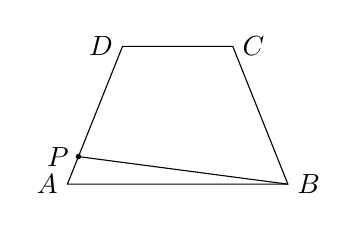
\begin{tikzpicture}[scale=0.7]
%\draw[help lines] (0,0) grid (4,4);
\draw (0,0) node[left](A){$A$} --(4,0)node[right](B){$B$} -- (3,2.5) node[right](C) {$C$}--(1,2.5) node[left](D){$D$}--cycle;
\coordinate[label=left:$P$] (P) at (0.2,0.5);
\draw[fill] (P) circle (1.1pt); 
\draw (P)--(4,0);
\end{tikzpicture}
\end{center}
\qs 设平面向量$ \vv{a},~\vv{b},~\vv{c} $均为非零向量,则“$ \vv{a}\bm\cdot\left(\vv{b}-\vv{c}\right)=0 $”是“$\vv{b}=\vv{c}$”的\xx
\twoch{充分而不必要条件}{必要而不充分条件}{充分必要条件}{既不充分也不必要条件}  
\qs 设$ E,~F $分别是正方形$ ABCD $的边$ AB,~BC $上的点,且$AE=\dfrac{1}{2}AB,~BF=\dfrac{2}{3}BC,~$如果$ \vv{EF}=m\vv{AB}+n\vv{AC}(m,n\text{为实数}) ,~$那么$ m+n $的值为\xx
\onech{$ -\dfrac{1}{2} $}{$0$}{$\dfrac{1}{2}$}{1}
\qs 若非零向量$ \bm{a,b} $满足$ \bm{a\cdot \left(a+b\right)}=0 ,\ 2\abs{\bm{a}}=\abs{\bm{b}}$,则向量$ \bm{a,\ b} $的夹角的大小为\tk.
\qs 在四边形$ ABCD $中,$ AB=2 $.若$ \vv{DA}=\dfrac{1}{2}\left(\vv{CA}+\vv{CB}\right) $,则$ \vv{AB}\cdot\vv{DC}= $\tk.
\qs 已知平面向量$\bm{a}$,$\bm{b}$满足$\bm{a}=\left(1,-1\right)$,~$\bm{\left(a+b\right)\bot\left(a-b\right)}$,那么$ \abs{\bm{b}}=\tk. $
\qs 已知$ M $为$\triangle ABC$所在平面内的一点,且$ \vv{AM}=\dfrac{1}{4}\vv{AB}+n\vv{AC}. $若点$ M $在$\triangle ABC$内部(不含边界),则实数$ n $的取值范围是\tk. 
\qs 如图,在直角梯形$ ABCD $中,$ AB\sslash CD,~AB\bot BC,~AB=2,~CD=1,~BC=a~(a>0),~ P$为线段$ AD $上一个动点,设$ \vv{AP}=x\vv{AD},~ \xl{PB}{PC}=y,~$对于函数$y=f(x),~$给出以下三个结论:\\
\ding{192} 当$ a=2 $时,函数$f(x)$的值域为$ \left[1,4\right] $;\\
\ding{193} $ \forall a\in\left(0,+\infty\right),~$都有$ f(1)=1 $成立;\\
\ding{194} $ \forall a\in\left(0,+\infty\right),~$函数$f(x)$的最大值都等于$ 4 $.\\
其中所有正确结论的序号是\tk.
\vspace{-7em}
\begin{flushright}
\begin{tikzpicture}[scale=1.2]
%\draw[help lines](0,0) grid (2.2,2.2);
\coordinate[label=below:$A$](A) at(0,0);
\coordinate[label=below:$B$](B) at(2,0);
\coordinate[label=left:$D$](D) at(1,2);
\coordinate[label=right:$C$](C) at(2,2);
\coordinate[label=left:$P$] (P) at($(A)!0.5!(D)$);
\draw (A)--(B)--(C)--(D)--cycle (B)--(P)--(C);
%\node(bq) at(2.1,0){$\text{图}1$};
\end{tikzpicture}
\end{flushright}
\qs 已知向量序列:$ \bm{a}_1,\bm{a}_2,\bm{a}_3,\cdots,\bm{a}_n,\cdots $满足如下条件:$ \left|\bm{a}_1\right|=4\left|\bm{d}\right|=2,~2\bm{a}_1\bm\cdot \bm{d}=-1 $且$ \bm{a}_n-\bm{a}_{n-1}=
\bm{d}~(n=2,3,4,\cdots). $若$ \bm{a}_1\bm{\cdot}\bm{a}_k=0,~ $则$ k= $\tk;~$ \left|\bm{a}_1\right|, \left|\bm{a}_2\right|, \left|\bm{a}_3\right|,\cdots, \left|\bm{a}_n\right|,\cdots$中第\tk 项最小.

\qs 如图,$ \triangle AB_1C_1,~\triangle C_1B_2C_2,~\triangle C_2B_3C_3 $是三个边长为2的等边三角形,且有一条边在同一直线上,边$ B_3C_3 $上有两个不同的点$ P_1,~P_2,~ $则$ \vv{AB_2}\bm{\cdot}(\vv{AP_1}+\vv{AP_2}) =$\tk.
\zj{
%\draw[help lines](0,0) grid (6,2);
\tikzmath{
\a=sqrt(3);
}
\coordinate[label=below:$A$](A) at (0,0);
\foreach \p in {1,2,3}
\coordinate[label=below:$C_{\p}$] (C_\p) at($(\p*2,0)$) ;
\foreach \q in {1,2,3}
\coordinate[label=above:$B_{\q}$] (B_\q) at($(2*\q-1,\a)$);
\foreach \r in{1,2,3}
\draw (B_\r)--(C_\r);
\draw (A)--(C_3) (A)--(B_1) (C_1)--(B_2) (C_2)--(B_3);
\draw[->,>=stealth] (A)--(B_2) ;
\draw[->,>=stealth](A)--($(B_3)!0.3!(C_3)$) node[right](P_1){$P_1$};
\draw[->,>=stealth](A)--($(B_3)!0.7!(C_3)$) node[right](P_2){$P_2$};
}

\end{questions}
\end{document}